\chapter{Εισαγωγή}
\label{ch:Introduction}

\section{Η ανάγκη για παράλληλα συστήματα} % Η εξέλιξη των σύγχρονων Η/Υ
\label{sec:The need for parallel systems}
Η βασική ιδέα της οργάνωσης των ηλεκτρονικών υπολογιστών με τη μορφή που αυτοί είναι γνωστοί έως και σήμερα, βασίζεται στην αρχιτεκτονική von Neumann όπως αυτή περιγράφηκε το 1945 από τον ουγγρικής και αμερικανικής καταγωγής μαθηματικό John von Neumann. Βάσει αυτής της περιγραφής, υπάρχει μία μονάδα επεξεργασίας η οποία επικοινωνεί με το τμήμα μνήμης, εκτελώντας εντολές και τροποποιώντας δεδομένα. Ο επεξεργαστής λαμβάνει μία-μία τις εντολές από τη μνήμη και τις εκτελεί προσπελαύνοντας ή/και τροποποιώντας δεδομένα που βρίσκονται στη μνήμη όταν αυτό καθορίζεται από την εντολή, με αυτό τον κύκλο να επαναλαμβάνεται συνεχώς. Το μοντέλο προγραμματισμού που χρησιμοποιείται στη συγκεκριμένη αρχιτεκτονική είναι γνωστό και ως σειριακό μοντέλο και φαίνεται στο Σχήμα X.

Η εποχή της πληροφορίας που ξεκίνησε στα μέσα του 20\textsuperscript{ού} αιώνα και οδήγησε σε μία οικονομία βασισμένη στην τεχνολογία της πληροφορίας, καθώς και η ολοένα και μεγαλύτερη χρήση των Η/Υ σε κάθε πτυχή της ζωής του ανθρώπου είχαν ως αποτέλεσμα την έναρξη ενός αγώνα ταχύτητας με σκοπό την κατασκευή όλο και πιο γρήγορων υπολογιστών.

Η κλιμάκωση της συχνότητας (frequency scaling) που αφορά την αύξηση της συχνότητας ενός επεξεργαστή με στόχο την επίτευξη μεγαλύτερης επίδοσης στα συστήματα που τον χρησιμοποιούν, αποτέλεσε τον κύριο λόγο αύξησης των επιδόσεων των εμπορικών Η/Υ από τα μέσα του 1980 έως και περίπου τα τέλη του 2004, όταν αυτή η προσπάθεια προσέκρουσε στο τείχος της ισχύος (power wall) όπως φαίνεται στο Σχήμα \ref{fig:CPUDB}. Αυτό συνέβει καθώς η αύξηση της συχνότητας οδήγησε στην αύξηση της καταναλισκόμενης ισχύος η οποία με τη σειρά της είχε ως αποτέλεσμα την αύξηση του κόστους λειτουργίας αλλά και την οδήγηση του υλικού στα όριά του με χαρακτηριστικό παράδειγμα την υπερθέρμανσή του.

\begin{figure}[t]
	\centering
	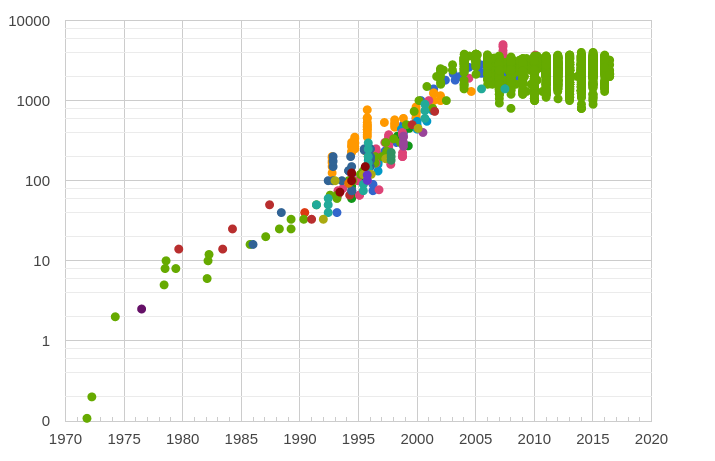
\includegraphics[width=0.7\textwidth]{Figures/cpudb.png}
	\linebreak 
	{\small (Η απεικόνιση προήλθε από την ιστοσελίδα του CPUDB \cite{danowitz2012cpu})}
	\caption{Η εξέλιξη της συχνότητας λειτουργίας (σε MHz) των μικροεπεξεργαστών.}
	\label{fig:CPUDB}
\end{figure}

%Η κλιμάκωση της συχνότητας (frequency scaling) αφορά την αύξηση της συχνότητας ενός επεξεργαστή με στόχο την επίτευξη μεγαλύτερης επίδοσης στα συστήματα που χρησιμοποιούν αυτόν τον επεξεργαστή. Η κλιμάκωση της συχνότητας αποτέλεσε την κινητήριο δύναμη που οδήγησε στην αύξηση των επιδόσεων των εμπορικών Η/Υ από τα μέσα του 1980 έως και περίπου τα τέλη του 2004, μέχρις ότου αυτή η προσπάθεια προσέκρουσε στο τείχος της ισχύος (power wall). Αυτό συνέβει καθώς η αύξηση της συχνότητας οδήγησε στην αύξηση της καταναλισκόμενης ισχύος η οποία με τη σειρά της οδήγησε σε μεγάλη κατανάλωση ρεύματος και υπερθέρμανση του υλικού.

Για να ξεπεραστεί το τείχος της ισχύος, οι κατασκευαστές των επεξεργαστών άρχισαν να ενσωματώνουν παραπάνω του ενός επεξεργαστικούς πυρήνες στο ίδιο ολοκληρωμένο κύκλωμα επεξεργαστή. Η αρχιτεκτονική αυτή βελτίωση είχε ως αποτέλεσμα τη γέννηση των πρώτων πολυπύρηνων (multicore) επεξεργαστών οι οποίοι έκαναν δυνατή την ταυτόχρονη εκτέλεση εντολών. Τα συστήματα που περιείχαν πολυπύρηνους επεξεργαστές αποτέλεσαν τα πρώτα εμπορικά μικρού μεγέθους παράλληλα συστήματα.

Στη σημερινή εποχή, τα πολυπύρηνα συστήματα είναι ευρέως διαδεδομένα καθώς απαντώνται από κινητά τηλέφωνα και ενσωματωμένους υπολογιστές χαμηλού κόστους και μεγέθους όσο μια πιστωτική κάρτα τραπέζης, μέχρι και υπολογιστικά συστήματα πολύ υψηλών επιδόσεων που διεξάγουν επιστημονικούς υπολογισμούς.


\section{Κατηγορίες Παράλληλων Συστημάτων}
\label{sec:Parallel System Categories}
Όταν μιλάμε για παράλληλα συστήματα ουσιαστικά αναφερόμαστε σε συστήματα που διαθέτουν μία συλλογή από επεξεργαστικές μονάδες που επικοινωνούν και συνεργάζονται για τη λύση ενός προβλήματος. Το πρόβλημα χωρίζεται σε επιμέρους εργασίες οι οποίες με τη σειρά τους ανατίθενται στις επεξεργαστικές μονάδες για εκτέλεση. Παρόλο που η ιδέα των πολλαπλών επεξεργαστικών μονάδων φαίνεται απλή, προκύπτουν ζητήματα τα οποία σχετίζονται πλην άλλων με τον τρόπο:
\begin{itemize}
	\item επικοινωνίας, συγχρονισμού και συντονισμού των επεξεργαστικών μονάδων
	\item διαμοιρασμού των εργασιών και
	\item προγραμματισμού ανάλογα με την οργάνωση του εκάστοτε συστήματος.
\end{itemize}
 
\subsection{Ταξινομία του Flynn}
Μία αρχική κατηγοριοποίηση των παράλληλων συστημάτων μπορεί να γίνει βάσει της ταξινομίας του Flynn και η οποία περιλαμβάνει τις εξής κατηγορίες:
\begin{itemize}
	\item SISD (single-instruction single-data) Σχήμα Χ
	\item SIMD (single-instruction multiple-data) Σχήμα Χ και
	\item MIMD (mutiple-instruction multiple-data) Σχήμα Χ
\end{itemize}

Στην κατηγορία SISD ανήκουν οι κλασικοί σειριακοί υπολογιστές οι οποίοι εκτελούν μία εντολή τη φορά (single-instruction) επάνω σε ένα δεδομένο (single-data). Στην κατηγορία SIMD συναντάμε επίσης υπολογιστές οι οποίοι εκτελούν μία εντολή τη φορά, αλλά μπορούν να την εφαρμόσουν ταυτόχρονα σε πολλαπλά δεδομένα (multiple-data) ώστε να εκμεταλλευτούν την παραλληλία επιπέδου δεδομένων (data-level parallelism). Τέλος, η κατηγορία MIMD θεωρείται ως η κατηγορία των καθαρά παράλληλων υπολογιστών οι οποίοι μπορούν και εκτελούν ταυτόχρονα πολλαπλές εντολές, με κάθε μία να ασχολείται με διαφορετικό δεδομένο.

Όπως θα δούμε στη συνέχεια, οι υπολογιστές MIMD, μπορούν να κατηγοριοποιηθούν περαιτέρω βάσει του πώς είναι οργανωμένη η μνήμη τους.

\subsection{Ταξινόμηση βάσει της οργάνωσης της μνήμης}
\label{ssec:Classification based on memory organization}
Η ταξινόμηση των παράλληλων υπολογιστών σχετικά με το πώς είναι οργανωμένη η μνήμη μπορεί να γίνει είτε βάσει της φυσικής οργάνωσης της μνήμης είτε βάσει της εικόνας/άποψης που έχει ο προγραμματιστής για αυτή.

Σχετικά με την πρώτη κατηγοριοποίηση, οι παράλληλοι υπολογιστές διακρίνονται σε υπολογιστές με (φυσικά) κοινόχρηστη μνήμη (γνωστοί και ως πολυεπεξεργαστές) και σε υπολογιστές με (φυσικά) κατανεμημένη μνήμη.

Όσον αφορά την εικόνα που έχει ο προγραμματιστής για την οργάνωση της μνήμης, οι υπολογιστές μπορούν να διαχωριστούν σε υπολογιστές με κοινόχρηστο και σε υπολογιστές με κατανεμημένο χώρο διευθύνσεων. Αξίζει να σημειωθεί ότι η εικόνα από προγραμματιστική άποψη δεν ταυτίζεται απαραίτητα με την φυσική οργάνωση της μνήμης καθώς με χρήση ειδικού λογισμικού ένα σύστημα με φυσικά κατανεμημένη μνήμη μπορεί να παρέχει κοινόχρηστο χώρο διευθύνσεων.


\subsubsection{Συστήματα κοινόχρηστης μνήμης}
Τα συστήματα κοινόχρηστης μνήμης (SMM - Shared Memory Machines \cite{rauber2010parallel}) αποτελούνται από επεξεργαστές, κοινόχρηστη μνήμη (γνωστή και ως καθολική) η οποία είναι καθολικά προσβάσιμη από όλους τους επεξεργαστές και ένα δίκτυο διασύνδεσης για την επικοινωνία των επεξεργαστών με τη μνήμη. Από άποψη φυσικής οργάνωσης, η μνήμη μπορεί να αποτελείται από περισσότερα του ενός τμήματα/μέρη (modules) τα οποία όμως παρέχουν έναν κοινόχρηστο χώρο διευθύνσεων που είναι προσβάσιμος από όλους τους επεξεργαστές. Οι επεξεργαστές επικοινωνούν, συνεργάζονται και ανταλλάσσουν δεδομένα διαβάζοντας ή γράφοντας σε κοινόχρηστες μεταβλητές που βρίσκονται αποθηκευμένες στη μνήμη.

Το δίκτυο διασύνδεσης επεξεργαστών-μνήμης μπορεί να είναι ένας απλός δίαυλος (bus), ένα διακοπτικό δίκτυο (π.χ. crossbar) ή κάποιο δίκτυο πολλαπλών επιπέδων (π.χ. Δίκτυο Δέλτα). Στην περίπτωση που το δίκτυο διασύνδεσης είναι δίαυλος, τότε αναφερόμαστε σε αυτά τα συστήματα ως Συμμετρικοί Πολυεπεξεργαστές (SMPs - Symmetric Multiprocessors). Οι Συμμετρικοί Πολεπεξεργαστές διαθέτουν μία κοινόχρηστη μνήμη η οποία απέχει εξίσου από όλους τους επεξεργαστές και συνεπώς χαρακτηρίζονται ως συστήματα ομοιόμορφης προσπέλασης μνήμης (UMA - Uniform Memory Access). Όπως είναι φυσικό, αν οι επεξεργαστές είναι πολυπύρηνοι και διαθέτουν ιεραρχία από πολύ μικρές αλλά ταυτόχρονα πολύ γρήγορες μνήμες γνωστές ως κρυφές μνήμες (caches), τότε ο κάθε πολυπύρηνος επεξεργαστής αποτελεί ένα σύστημα SMP καθώς η πρόσβαση στην κρυφή μνήμη είναι πιο γρήγορη από την πρόσβαση στην κύρια μνήμη μέσω του διαύλου.

Επειδή το εύρος ζώνης (bandwidth) του διαύλου είναι σταθερό ανεξάρτητα από το πλήθος των επεξεργαστών που είναι συνδεδεμένοι σε αυτόν, όσο πιο πολλοί επεξεργαστές είναι συνδεδεμένοι, τόσο πιο πολύ υποβαθμίζεται η αποδοτικότητα του δικτύου λόγω των συγγρούσεων πρόσβασης στο κοινό μέσο και συνεπώς τόσο περισσότερο καθυστερεί η εξυπηρέτηση προσπελάσεων στη μνήμη, αυξάνοντας έτσι τον σχετικό (effective) χρόνο προσπέλασης. Για την αποδοτική υποστήριξη μεγαλύτερου αριθμού επεξεργαστών καταφεύγουμε στη χρήση κρυφής μνήμης ή άλλου τύπου δίκτυου διασύνδεσης.

Παράλληλα συστήματα μεγαλύτερου μεγέθους μπορούν να υλοποιηθούν χρησιμοποιώντας Συμμετρικούς Πολυεπεξεργαστές ως κόμβους ενός δικτύου διασύνδεσης (Σχήμα Χ). Σε αυτά τα συστήματα καθίσταται δυνατή η παροχή ενός κοινόχρηστου χώρου διευθύνσεων με χρήση κατάλληλων πρωτοκόλλων συνοχής τα οποία αποκρύπτουν από τον χρήστη του συστήματος την κατανεμημένη οργάνωση της φυσικής μνήμης. Η αρχιτεκτονική που μόλις περιγράφηκε είναι γνωστή και ως κατανεμημένη κοινόχρηστη μνήμη (DSM - Distrubuted Shared Memory), ενώ τα συστήματα αυτά ονομάζονται συστήματα ανομοιόμορφης προσπέλασης μνήμης (NUMA - Non-Uniform Memory Access). Σε περίπτωση ύπαρξης ιεραρχίας κρυφών μνημών στους κόμβους (Σχήμα Χ), χρειάζεται η χρήση ενός πρωτοκόλλου συνοχής κρυφής μνήμης (cache coherence protocol) το οποίο θα εξασφαλίζει ανά πάσα στιγμή ότι οποιαδήποτε προσπέλαση μνήμης θα επιστρέφει την πιο πρόσφατη τιμή. Τέτοια συστήματα είναι γνωστά ως cc-NUMA (Cache coherent NUMA).

\subsubsection{Συστήματα κατανεμημένης μνήμης}
Τα συστήματα κατανεμημένης μνήμης (DMM - Distributed Memory Machines) αποτελούνται από επεξεργαστικά στοιχεία (γνωστά ως κόμβοι) και από ένα δίκτυο διασύνδεσης το οποίο επιτρέπει την επικοινωνία μεταξύ των κόμβων (Σχήμα Χ). Κάθε κόμβος περιέχει επεξεργαστή, τοπική μνήμη και ίσως περιφερειακές συσκευές. Η τοπική μνήμη κάθε κόμβου είναι απευθείας προσβάσιμη μόνο από τον επεξεργαστή του ίδιου κόμβου, ενώ όταν κάποιος επεξεργαστής χρειάζεται να προσπελάσει την τοπική μνήμη που βρίσκεται σε κάποιον άλλο κόμβο, αυτό επιτυγχάνεται με μεταβίβαση μηνυμάτων μέσω του δικτύου διασύνδεσης. 

Συλλογές υπολογιστών που είναι συνδεδεμένοι μέσω δικτύου διασύνδεσης αφιερωμένου αποκλειστικά στη μεταξύ τους επικοινωνία ονομάζονται συστάδες (clusters). Οι συστάδες υπολογιστών χρησιμοποιούνται ευρέως λόγω της διαθεσιμότητας δικτύων διασύνδεσης υψηλών επιδόσεων όπως το Switched Gigabit Ethernet, το Infiniband, το Myriret κ.ά. Πολλαπλές συστάδες υπολογιστών μπορούν να διασυνδεθούν μεταξύ τους και να δημιουργήσουν συστήματα πλέγματος (grids).

Το πλήθος των κόμβων και το πλήθος των επεξεργαστών στα συστήματα κατανεμημένης μνήμης μπορεί να φτάσει τις εκατοντάδες χιλιάδες και κάποια εκατομμύρια αντίστοιχα, σε αντίθεση με τα συστήματα κοινόχρησης μνήμης όπου το πλήθος των επεξεργαστών περιορίζεται σε μερικές δεκάδες. Προφανώς, η ικανότητα κλιμάκωσης των κατανεμημένων συστημάτων εξαρτάται από την σωστή επιλογής της τοπολογίας του δικτύου διασύνδεσης.


\section{Προγραμματισμός Παράλληλων Συστημάτων}

\subsection{Συστήματα κοινόχρηστης μνήμης}
\label{ssec:Shared Memory Programming}
Ο προγραμματισμός των συστημάτων κοινόχρηστης μνήμης συνήθως βασίζεται στη χρήση νημάτων, δηλαδή σε ξεχωριστές ακολουθίες ελέγχου (στοίβα + μετρητής προγράμματος) που μοιράζονται δεδομένα με τα υπόλοιπα  νήματα μέσω κοινόχρηστου χώρου διευθύνσεων. Η ύπαρξη κοινόχρηστων δεδομένων εγείρει ζητήματα όπως αυτό της ταυτόχρονης προσπέλασής τους από διαφορετικά νήματα, καθώς κάτι τέτοιο θα μπορούσε να οδηγήσει σε συνθήκες ανταγωνισμού (race conditions). Όταν υπάρχουν συνθήκες ανταγωνισμού, το τελικό αποτέλεσμα των ταυτόχρονων προσπελάσεων μνήμης εξαρτάται από τις σχετικές ταχύτητες εκτέλεσεις των νημάτων. Για την αποφυγή συνθηκών ανταγωνισμού και την εξασφάλιση της ακεραιότητας των δεδομένων χρησιμοποιείται ο αμοιβαίος αποκλεισμός (mutual exclusion), βάσει του οποίου μόνο ένα νήμα κάθε φορά μπορεί να εκτελεί εντολές που τροποποιούν κοινόχρηστες μεταβλητές.

Η πιο διαδεδομένη βιβλιοθήκη νημάτων και μοντέλο εκτέλεσης είναι αυτό των POSIX threads (pthreads) το οποίο παρέχει κλήσεις διαχείρισης (π.χ. δημιουργία, τερματισμό) νημάτων, κλειδαριές (mutexes), μεταβλητές συνθήκης (condition variables) και κλήσεις συγχρονισμού νημάτων όπως για παράδειγμα κλήσεις φραγής (barriers). Ο προγραμματιστής έχει την πλήρη ευθύνη για τη δημιουργία των νημάτων, την ανάθεση εργασιών σε αυτά, προεραιτικά την αντιστοίχηση των νημάτων σε επεξεργαστές, πιθανώς την συλλογή των επιμέρους αποτελεσμάτων και την σύνθεση του τελικού αποτελέσματος από αυτά, καθώς και τον τερματισμό τους. Επιπλέον, είναι υπεύθυνος για τον συγχρονισμό των νημάτων και την αποφυγή συνθηκών ανταγωνισμού με χρήση κατάλληλων προγραμματιστικών δομών.

Για τη διευκόλυνση του προγραμματισμού, έχουν αναπτυχθεί εργαλεία πιο υψηλού επιπέδου όπως το OpenMP (Open Multi-Processing). Το OpenMP είναι μία διεπαφή προγραμματισμού εφαρμογών (API - Application Programming Interface) η οποία αποτελείται από οδηγίες (directives) προς τον μεταφραστή, ρουτίνες βιβλιοθήκης και μεταβλητές περιβάλλοντος (environment variables) και συντελεί στην συγγραφή πολυνηματικού κώδικα για συστήματα κοινόχρηστης μνήμης. Πολύ σημαντικό είναι το γεγονός ότι το OpenMP δίνει τη δυνατότητα παραλληλοποίησης του υπάρχοντα σειριακού κώδικα χωρίς την τροποποίησή του, παρά μόνο με την προσθήκη των ειδικών οδηγιών οι οποίες μπορούν να αγνοηθούν σε περίπτωση που δεν υποστηρίζονται από κάποιο μεταφραστή. Επίσης, η διαχείριση των νημάτων γίνεται αυτόματα, ενώ όλα τα υπόλοιπα ζητήματα που σχετίζονται με τον συγχρονισμό, ανάθεση εργασιών κλπ απλοποιούνται σε μεγάλο βαθμό. Η απλότητα του OpenMP αλλά και όλες οι διευκολύνσεις που προσφέρει, το κάνουν να βρίσκεται στην κορυφή των προτιμήσεων για προγραμματισμό συστημάτων κοινόχρηστης μνήμης, αφού μπορεί να χρησιμοποιηθεί ακόμα και από προγραμματιστές χωρίς ιδιαίτερη εμπειρία ή γνώσεις σχετικές με την παράλληλη επεξεργασία. Περισσότερα για το πρότυπο OpenMP θα ειπωθούν στο Κεφάλαιο \ref{ch:OpenMP API}.


\subsection{Συστήματα κατανεμημένης μνήμης}
Ο προγραμματισμός των συστημάτων κατανεμημένης μνήμης συνήθως βασίζεται στη μεταβίβαση μηνυμάτων μεταξύ αυτόνομων διεργασιών (προγράμματα υπό εκτέλεση) οι οποίες βρίσκονται σε διαφορετικούς κόμβους και δεν μοιράζονται κοινόχρηστες μεταβλητές, αλλά πραγματοποιούν μεταξύ τους αποστολή και λήψη μηνυμάτων. Η μη ύπαρξη κοινόχρηστων δεδομένων εξαλείφει την ανάγκη για αμοιβαίο αποκλεισμό αλλά ταυτόχρονα δυσκολεύει τον συγχρονισμό μεταξύ των διεργασιών. Ο προγραμματιστής είναι υπεύθυνος να καθορίσει πότε σταματούν οι υπολογισμοί και πότε ξεκινούν οι επικοινωνίες, το περιεχόμενο, τον αποστολέα και τους παραλήπτες των μηνυμάτων, καθώς και να αποφασίσει τον τύπο της επικοινωνίας που θα χρησιμοποιήσει (σύγχρονη ή ασύγχρονη).

Στις σύγχρονες επικοινωνίες μία διεργασία που θέλει να στείλει (λάβει) δεδομένα μπλοκάρει στην αντίστοιχη κλήση αποστολής (λήψης) μέχρις ότου η διαδικασία παραλήπτης (αποστολέας) παραλάβει (αποστείλει) τα δεδομένα. Ο τρόπος λειτουργίας των σύγχρονων επικοινωνιών τις καθιστά ιδανικές για την επίτευξη συγχρονισμού μεταξύ των διεργασιών. Αντίθετα, στις ασύγχρονες επικοινωνίες, η διεργασία δεν μπλοκάρει αλλά συνεχίζει κανονικά την εκτέλεση της.

Λόγω της φύσης του μοντέλου μεταβίβασης μηνυμάτων, ο προγραμματιστής θα πρέπει να δώσει προσοχή στο πώς θα ελαχιστοποιήσει την επικοινωνία μεταξύ διαφορετικών κόμβων, καθώς η προσπέλαση της τοπικής μνήμης κάθε κόμβου είναι πολύ πιο γρήγορη απ' ότι η προσπέλαση της μνήμης άλλων κόμβων. Γι' αυτό το λόγο πρέπει να σχεδιαστεί με σύνεση ο διαμοιρασμός των δεδομένων ανάμεσα στους κόμβους, καθώς και η ανάθεση φόρτου σε κάθε διεργασία ώστε εκτός από την αποφυγή καθυστερήσεων σε απομακρυσμένες προσπελάσεις, να αποφευχθεί και συμφόρηση του δίκτυου.

Δημοφιλές πρότυπο μεταβίβασης μηνυμάτων αποτελεί το MPI (Message Passing Interface) με τις δύο πιο γνωστές υλοποιήσεις του να είναι το Open MPI και το MPICH. Το MPI υποστηρίζει τη μεταβίβαση μηνυμάτων στις γλώσσες C, C++ και Fortran με στόχο την ανάπτυξη μεταφέρσιμων παράλληλων εφαρμογών μεγάλης κλίμακας. Μεγάλο προτέρημα αποτελεί η απόκρυψη των πληροφοριών χαμηλού επιπέδου όπως ο τύπος του υποκείμενου δικτύου, το λειτουργικό σύστημα του κάθε κόμβου, αλλά και η ύπαρξη βοηθητικών προγραμματιστικών δομών, όπως οι συλλογικές και μη επικοινωνίες που μπορούν να πραγματοποιηθούν χωρίς τη γνώση δικτυακού προγραμματισμού (sockets).


\section{Αντικείμενο της Διπλωματικής Εργασίας}
\label{sec:Subject of the Diploma Thesis}
Το αντικείμενο της παρούσας διπλωματικής εργασίας είναι η επίτευξη καλύτερων επιδόσεων στον ερευνητικό μεταφραστή OMPi, μέσω της εκμετάλλευσης πληροφοριών που σχετίζονται με την τοπολογία του συστήματος. Ο OMPi είναι ένας μεταφραστής πηγαίου σε πηγαίο κώδικα (source-to-source) που υποστηρίζει τη διεπαφή προγραμματισμού εφαρμογών OpenMP και αναπτύσσεται από την Ομάδα Παράλληλης Επεξεργασίας του Πανεπιστημίου Ιωαννίνων.

Στην έκδοση 4.0 του OpenMP προστέθηκε η δυνατότητα ανάθεσης (binding) των νημάτων σε σύνολα από συγκεκριμένους επεξεργαστές (τα λεγόμενα OpenMP places) ώστε να εκτελεστούν σε αυτά. Η ανάθεση των νημάτων σε OpenMP places γίνεται βάσει των διάφορων διαθέσιμων πολιτικών (γνωστές ως processor binding policies). Ο χρήστης έχει τη δυνατότητα προσδιορισμού της λίστας των διαθέσιμων OpenMP places αλλά και της πολιτικής ανάθεσης των νημάτων σε αυτά. Στο OpenMP 5.1 (Νοέμβριος 2020) επεκτάθηκαν περαιτέρω οι τρόποι προσδιορισμού των OpenMP places οι οποίοι περιγράφονται με λεπτομέρεια στην Ενότητα \ref{sec:Topology in OpenMP}. Στα πλαίσια της διπλωματικής εργασίας υλοποιήθηκε πλήρης υποστήριξη των προαναφερθέντων λειτουργιών και οι οποίες συμμορφώνονται με τις προδιαγραφές του OpenMP 5.1.

Επιπρόσθετα, ανεξάρτητα από το πρότυπο OpenMP, έγινε εκμετάλλευση της τοπολογίας για τη βελτίωση των κλήσεων φραγής που υλοποιούνται στο μεταφραστή OMPi. Συγκεκριμένα, σε περίπτωση που αναγνωρίζεται το υποκείμενο σύστημα ως σύστημα ανομοιόμορφης προσπέλασης μνήμης (NUMA), τότε εφαρμόζεται ένας νέος αλγόριθμος για τις κλήσεις φραγής που λαμβάνει υπόψην του την τοπολογία για την επίτευξη ταχύτερου συγχρονισμού των νημάτων.


\section{Διάρθρωση της Διπλωματικής Εργασίας}
\label{sec:Structure of the Diploma Thesis}
Η διπλωματική εργασία είναι οργανωμένη με τον ακόλουθο τρόπο:
\begin{itemize}
	\item Κεφάλαιο 2: Παρουσίαση της διεπαφής προγραμματισμού εφαρμογών OpenMP και περιγραφή της σύνταξης των πιο διαδεδομένων οδηγιών. % που καλύπτουν τις ανάγκες της πλειοψηφίας των εφαρμογών.
	Αναφορά στους διάφορους μεταφραστές που υποστηρίζουν το OpenMP και περιγραφή του μεταφραστή OMPi.
	\item Κεφάλαιο 3: Εισαγωγή στην τοπολογία, περιγραφή των συστημάτων NUMA, εργαλεία για την αναγνώριση και εκμετάλλευση της τοπολογίας και η χρήση της τελευταίας στα πλαίσια του OpenMP. Παρουσίαση των λειτουργιών του OpenMP που σχετίζονται με την τοπολογία και υλοποιήθηκαν στον μεταφραστή OMPi.
	\item Κεφάλαιο 4: Περιγραφή του τρόπου επίτευξης συγχρονισμού με χρήση κλήσεων φραγής (barriers) και παρουσίαση των ιδιαίτερων χαρακτηριστικών τους στα πλαίσια του OpenMP. Επεξήγηση της υλοποίησης των κλήσεων φραγής στον μεταφραστή OMPi και των βελτιώσεων που έγιναν για την επίτευξη καλύτερων επιδόσεων σε πολυπύρηνα συστήματα NUMA.
	\item Κεφάλαιο 5: Παρουσίαση και ανάλυση των αποτελεσμάτων από την εκτέλεση διάφορων πειραμάτων για τη μέτρηση της απόδοσης του μεταφραστή OMPi μετά την υλοποίηση των λειτουργιών που σχετίζονται με την τοπολογία και των βελτιώσεων στις κλήσεις φραγής.
	\item Κεφάλαιο 6: Σύνοψη της διπλωματικής εργασίας και αναφορά σε μελλοντικές εργασίες.
\end{itemize}

